\chapter{Results validation}
\label{ch:simu_expe}

This chapter presents the simulations and the first experimental tests carried out to validate the behavior of the drone show. The main objective was to verify the stability of the trajectories, the consistency of the selected formations, and the ability of the drones to satisfy the safety constraints, especially obstacle avoidance and the preservation of sufficient distances between vehicles.

After several preliminary tests with the available models, we observed that the Crazyflie CF2 drones were the most stable for our case study. Their flight behavior was more regular and predictable, which made it easier to execute the planned trajectories. For this reason, we decided to continue the simulations and experimental tests using only CF2 drones.

The work was mainly organized through GitHub. Each group member developed their own part of the demonstration, working on trajectories, formations, or simulation scripts. The different contributions were then merged at the end in order to obtain a common and coherent version of the project.

Many simulations were carried out before the real flight tests. As shown in the following figures, several configurations were tested to ensure obstacle avoidance, separation between drones, and the visual quality of the show. The formations were selected not only to validate the technical aspects, but also to achieve a satisfactory level of spectacle.

\begin{figure}[H]
    \centering
    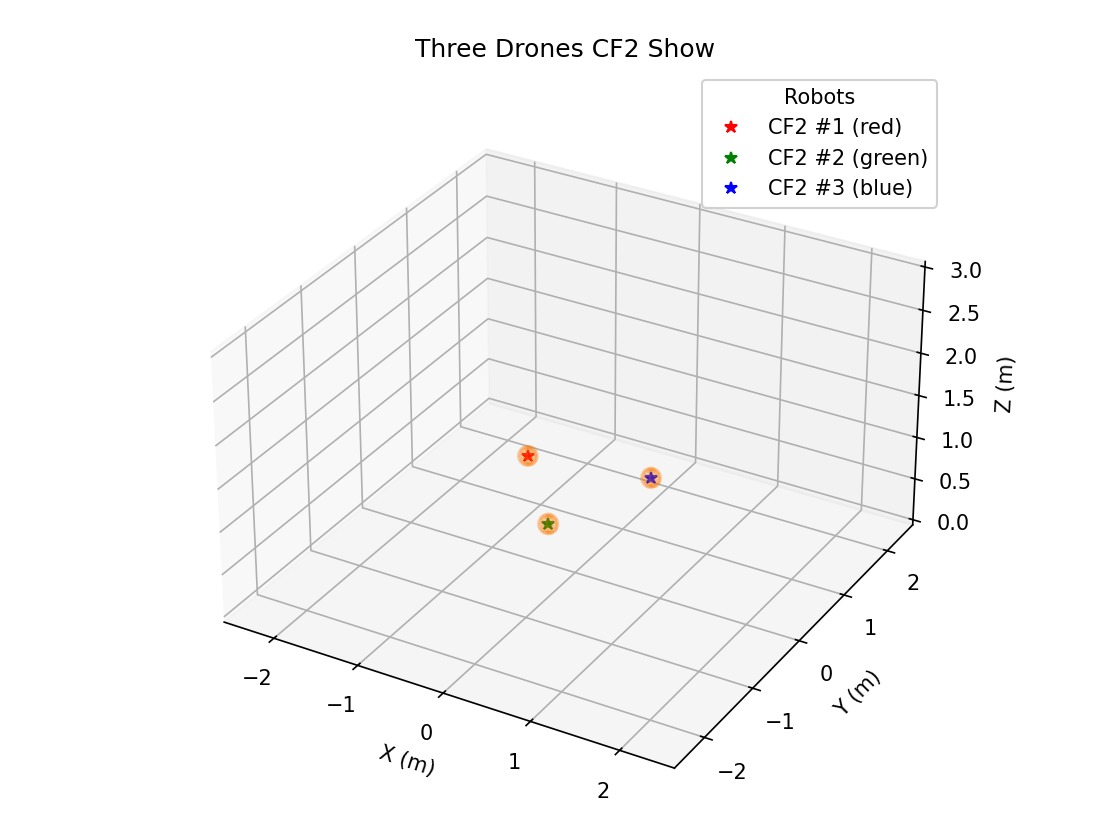
\includegraphics[width=0.8\textwidth]{prism-uploads/WhatsApp Image 2026-05-30 at 13.13.25.jpeg}
    \caption{Three-drone simulation in a triangular formation.}
    \label{fig:simu_3drones_triangle}
\end{figure}

\begin{figure}[H]
    \centering
    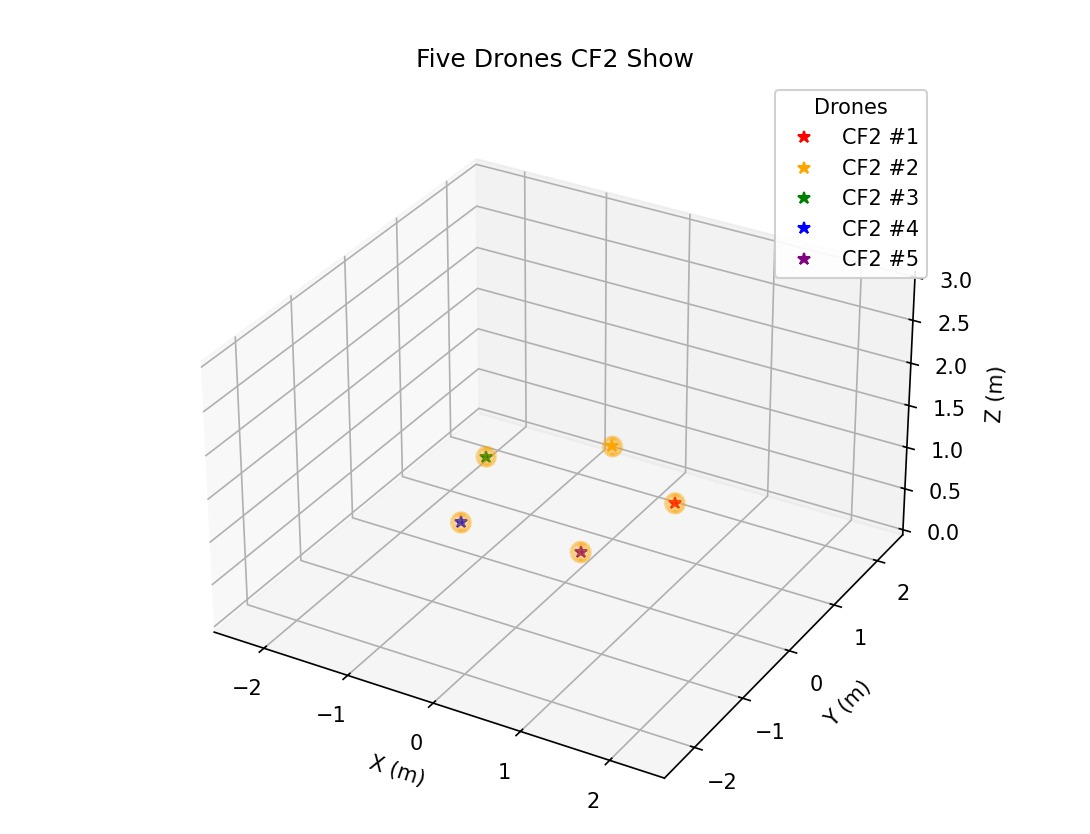
\includegraphics[width=0.8\textwidth]{prism-uploads/WhatsApp Image 2026-05-30 at 13.14.47_2.jpeg}
    \caption{Five-drone simulation in a horizontal pentagon formation.}
    \label{fig:simu_5drones_pentagone_horizontal}
\end{figure}

\begin{figure}[H]
    \centering
    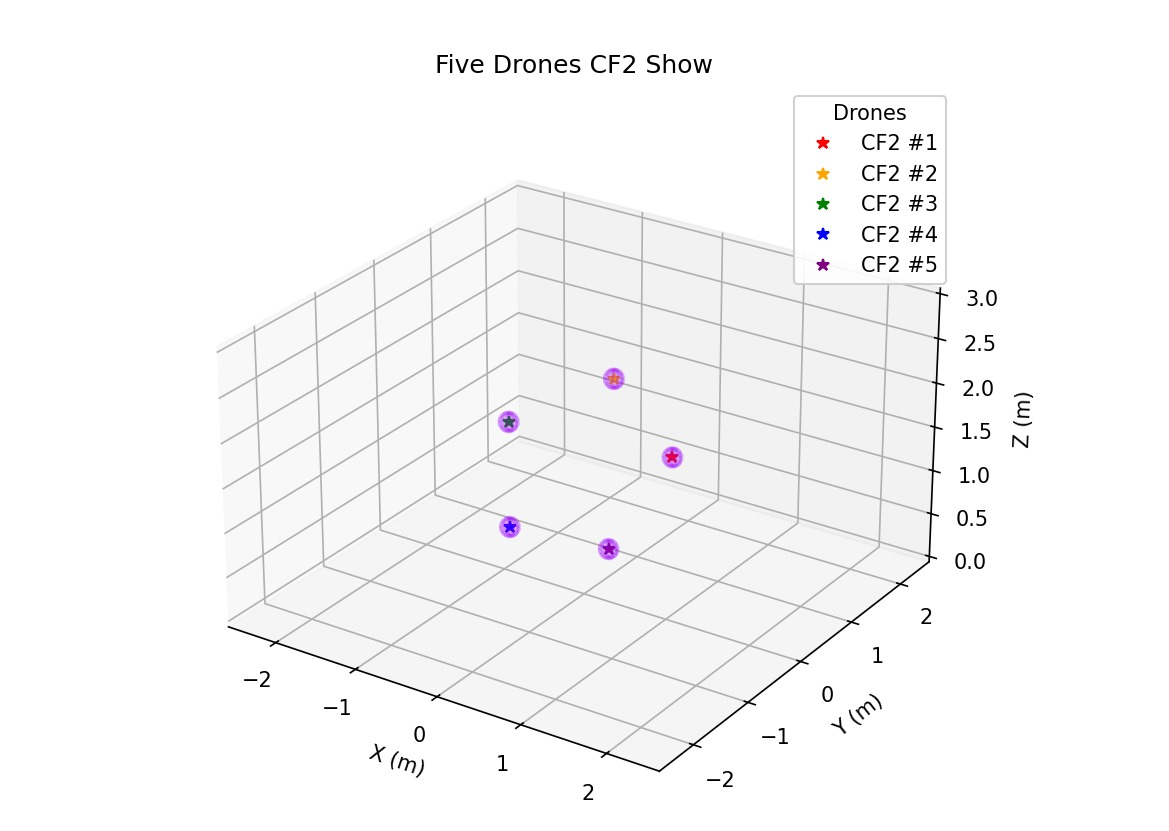
\includegraphics[width=0.8\textwidth]{prism-uploads/WhatsApp Image 2026-05-30 at 13.12.14.jpeg}
    \caption{Five-drone simulation in a vertical pentagon formation.}
    \label{fig:simu_5drones_pentagone_vertical}
\end{figure}

An initial real test with three drones was successfully performed in the flight arena on 27/05. This test confirmed that the simulated trajectories could be transferred to a real experimental environment while maintaining good flight stability. Additional tests with five and seven drones were then planned for 01/06 in order to evaluate the transition to a larger fleet and to validate more complex formations.

\begin{figure}[H]
    \centering
    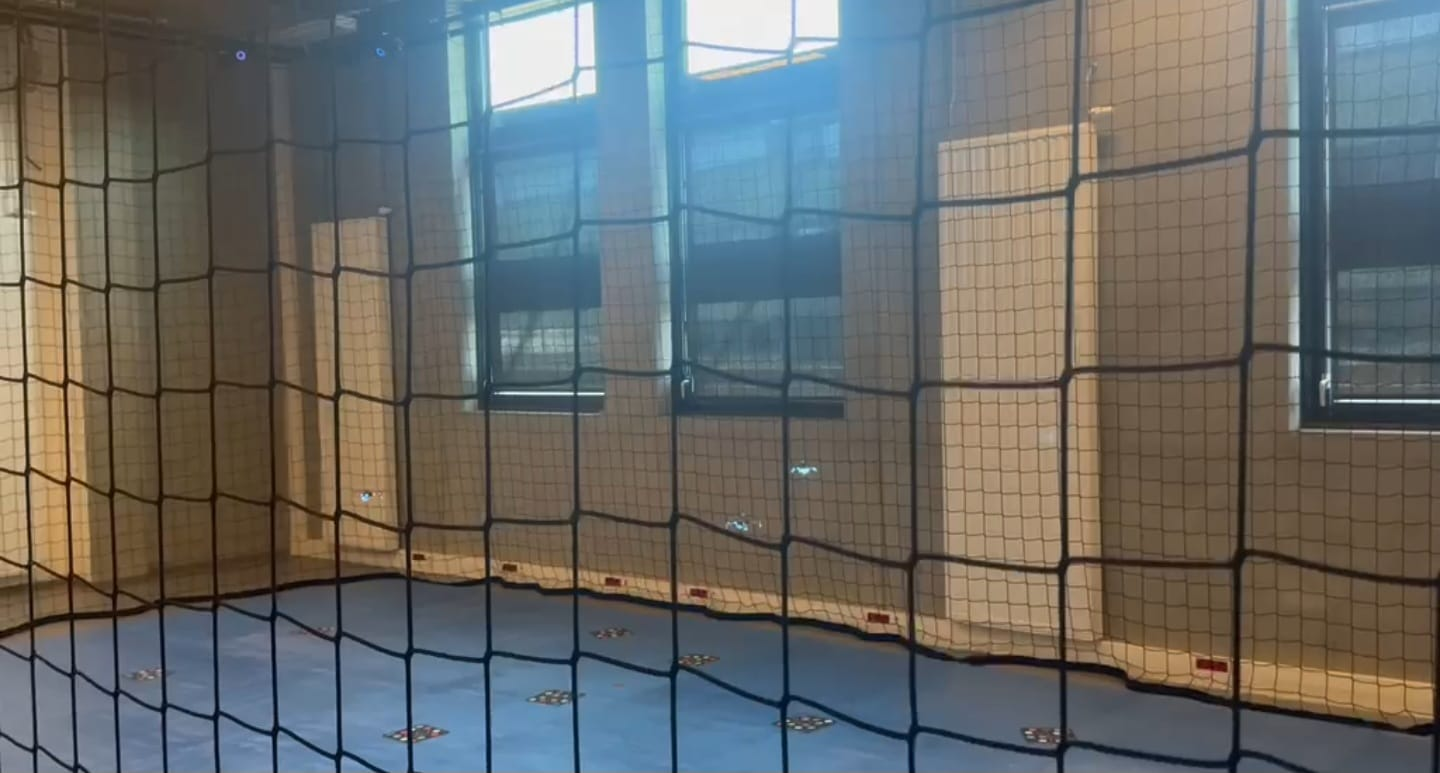
\includegraphics[width=0.85\textwidth]{prism-uploads/WhatsApp Image 2026-05-30 at 13.06.01.jpeg}
    \caption{Real test with three drones in the flight arena.}
    \label{fig:test_reel_3drones_voliere}
\end{figure}


As a future improvement, we also considered making the drone show more interactive. One possible extension would be to allow a user to draw a shape or trajectory on a tablet, with the drones responding to this input almost in real time. In this scenario, the drawing would be converted into reference points or trajectories, and the fleet would adapt its formation accordingly. This idea was not implemented in the current version, but it represents an interesting direction for future work, combining trajectory generation, user interaction, and real-time control.
